
\section{Preliminaries}
\anibal{does $R$ have to be commutative?}

For the rest of this work we fix a commutative ring with unit $R$ and work over its associated symmetric monoidal category $(\Ch, \otimes, R)$ of chain complexes.
As usual, we regard the set of $R$-linear maps $\Hom(C, C^\prime)$ between chain complexes as a chain complex.
The $i\th$ suspension functor $s^i \colon \Ch \to \Ch$ is defined on objects by $(s^{i}C)_n= C_{n-i}$.

A \textit{coassociative counital coalgebra} $C = (C, \partial, \Delta, \varepsilon)$ is the data of an object $(C, \partial) \in \Ch$ equipped with maps $\Delta \colon C \to C \otimes C$ and $\varepsilon \colon C\to R$ in $\Ch$ satisfying the usual coassociativity and counitality relations. 
This notion is equivalent to that of a comonoid in $(\Ch, \otimes, R)$. Denote by $\coAlg$ the category of coassociative counital coalgebra with morphisms being structure preserving chain maps. 
It is a symmetric monoidal category $(\coAlg, \otimes, R)$ with structure maps:
\begin{equation} \label{e:coalgebras are symmetric monoidal1}
\begin{tikzcd}
C \otimes C^\prime \arrow[r, "\Delta \otimes \Delta^\prime"] &
(C \otimes C) \otimes (C^\prime \otimes C^\prime) \arrow[r, "(23)"] &
(C \otimes C^\prime) \otimes (C \otimes C^\prime),
\end{tikzcd}
\end{equation}
\begin{equation} \label{e:coalgebras are symmetric monoidal2}
\begin{tikzcd}
C \otimes C^\prime \arrow[r, "\varepsilon \otimes \varepsilon^\prime"] &
R \otimes R \arrow[r, "\cong"] & R.
\end{tikzcd}
\end{equation}

We will denote the category of monoids in a monoidal category $\C$ by $\Mon_{\C}$.\footnote{Monoids in $\Ch$ and $\coAlg$ are sometimes referred to as dg associative unital algebras and dg bialgebras respectively, but we avoid this terminology.}




\subsection{The cobar construction}

Let $C$ be a coassociative counital coalgebra. A \textit{coaugmentation} is a morphism $\nu \colon R \to C$ in $\coAlg$.
Denote by $\coAlg^*$ the category of coaugmented coassociative counital coalgebras with morphisms being coaugmentation preserving morphisms in $\coAlg$. 

We recall the definition of the \textit{cobar} functor 
$$ \cobar \colon \coAlg^* \to \Mon_{\Ch}.$$

Let  $(C, \partial, \Delta, \varepsilon, \nu)  \in \coAlg^*$ where $\nu \colon R \to C$ is the coaugmentation. Define
$$ \cobar(C, \partial, \Delta, \varepsilon, \nu)  \colon= ( T(s^{-1}  \overline{C} ), D, \mu) \in \Mon_{\Ch}$$ where 
\begin{itemize}
\item $\overline{C}=\text{coker}(\nu \colon R \to C)$
\item $T(s^{-1} \overline{C})= R \oplus \overline{C} \oplus (\overline{C}  \otimes \overline{C} ) \oplus ( \overline{C} \otimes \overline{C} \otimes \overline{C} ) \oplus\cdots $
\item $\mu \colon T(s^{-1}  \overline{C} )^{\otimes 2} \to T(s^{-1}  \overline{C} ) $ is the free associative unital product given by concatenation of monomials
\item $D \colon T(s^{-1}  \overline{C} ) \to T(s^{-1}  \overline{C} )$ is the derivation of degree $-1$ determined by extending the linear map $$- s^{-1} \circ \partial \circ s^{+1} + (s^{-1} \otimes s^{-1}) \circ \Delta \circ s^{+1} \colon s^{-1}\overline{C} \to s^{-1}\overline{C} \oplus (s^{-1}\overline{C} \otimes s^{-1}\overline{C}) \hookrightarrow T(s^{-1}C)$$ as a derivation.
\end{itemize}

The coassociativity of $\Delta$, the compatibility of $\partial$ and $\Delta$, and the fact that $\partial^2 =0$ together imply that $D^2=0$. This construction is clearly functorial with respect to maps in $\coAlg^*$. We will denote $ \cobar (C, \partial, \Delta, \varepsilon, \nu)$ simply by $ \cobar(C)$. 

In this article we are mostly concerned with \textit{connected} coalgebras, namely coaugmented coalgebras $C \in \coAlg^*$ which are non-negatively graded and the coaugmentation $\nu \colon R \to C$ induces an isomorphism of coalgebras $R \cong C_0$. We denote by $\coAlg^0$ the full subcategory of $\coAlg^*$ consisting of connected coalgebras. If $C \in \coAlg^0$, then $ \cobar(C)$ is concentrated on non-negative degrees. 

The cobar construction was originally applied by Adams' to the coalgebra of normalized chains on a $1$-reduced simplicial set to obtain a model for the chains on the based loop space \cite{Adams}. The cobar construction as a model for the based loop space was furthered studied in \cite{Baues} and more recently, in the non-simply connected setting in \cite{Hess-Tonks}, \cite{Rivera-Zeinalian}.

%\section{The prop $\M$}

\subsection{Operads and props} \label{s:operads and props}

Let $\S$ be the category whose objects are the natural numbers and whose set of morphisms between $m$ and $n$ is empty if $m \neq n$ and is otherwise the symmetric group $\S_n$.
A \textit{left $\S$-module} (resp. \textit{right} $\S$-\textit{module} or $\S$-\textit{bimodule}) is a covariant functor from $\S$ (resp. $\S^\op$ or $\S \times \S^\op$) to $\Ch$.
In this paper we prioritize left module structures over their right counterparts. As usual, taking inverses makes both perspectives equivalent.
We respectively denote by $\smod$ and $\sbimod$ the categories of left $\S$-modules and of $\S$-bimodules with morphisms given by natural transformations.

The collections of group homomorphism $\S_n \to \S_n \times \S_1$ for $n \geq 0$ induces a forgetful functor $U \colon \sbimod \to \smod$.
The similarly defined forgetful functor to right $\S$-modules will not be used.

Given an object $C$ in $\C$ define:
\begin{align*}
\End^C(r) &= \Hom(C, C^{\otimes r}),
&\End^C_C(r, s) &= \Hom(C^{\otimes r}, C^{\otimes s}),
\end{align*}
with their natural structures of $\S$-module and $\S$-bimodule respectively.
The forgetful functor $U$ sends $\End^C_C$ to $\End^C$.

We can define \textit{operads} and \textit{props} by enriching $\S$-modules and \mbox{$\S$-bimodules} with certain composition structures.
For a complete presentation of these concepts we refer to Definition 11 and 54 of \cite{Markl08}.
Intuitively, operads and props can be understood by abstracting the composition structure naturally present in the left $\S$-module $\End^C$, naturally an operad, and the $\S$-bimodule $\End^C_C$, naturally a prop.
We remark that the structure on a prop $\P$ restricts to an operad structure on $U(\P)$.

We can also think of operads and props as algebras over the monad associated to the free-forgetful adjunctions
\begin{equation*}
\begin{tikzcd}
\smod \arrow[r, bend left] & \arrow[l, bend left] \operads 
& \text{and} &
\sbimod \arrow[r, bend left] & \arrow[l, bend left] \props
\end{tikzcd}
\end{equation*}
which we now review, see \cite{Markl08} or \cite{Fresse2010props} for a more detailed presentation.

The \textit{free prop} $F(M)$ generated by an \mbox{$\S$-bimodule} $M$ is constructed using open directed graphs with no directed loops that are enriched with a labeling described next. We think of each directed edge as built from two compatibly directed half-edges. For each vertex $v$ of a directed graph $G$, we have the sets $in(v)$ and $out(v)$ of half-edges that are respectively incoming to and outgoing from $v$. Half-edges that do not belong to $in(v)$ or $out(v)$ for any $v$ are divided into the disjoint sets $in(G)$ and $out(G)$ of incoming and outgoing external half-edges. For any positive integer $n$ let $\overline{n} = \{1,\dots,n\}$ and set $\overline{0} = \emptyset$. For any finite set $S$, denote the cardinality of $S$ by $|S|$. The labeling is given by bijections  
\begin{equation*}
\overline{|in(G)|}\to in(G), \qquad
\overline{|out(G)|}\to out(G),
\end{equation*}
and
\begin{equation*}
\overline{|in(v)|}\to in(v), \qquad
\overline{|out(v)|}\to out(v),
\end{equation*}
for every vertex $v$.
We refer to the isomorphism classes of such labeled directed graphs with no directed loops as $(n,m)$\textit{-graphs} denoting the set of these by $\G(m,n)$.
We use graphs immersed in the plane to represent elements in $\G(m,n)$, please see Figure \ref{f:immersion}.
We consider the right action of $\S_n$ and the left action of $\S_m$ on a $(n,m)$-graph given respectively by permuting the labels of $in(G)$ and $out(G)$. This action defines the $\S$-bimodule structure on the free prop
\begin{equation} \label{e:free prop}
F(M)(m,n) \ = \bigoplus_{\Gamma \in \G(m,n)} \bigotimes_{v \in Vert(\Gamma)} out(v) \otimes_{\S_q} M(p, q) \otimes_{\S_p} in(v),
\end{equation}
where we simplified the notation writing $p$ and $q$ for $\overline{|in(v)|}$ and $\overline{|out(v)|}$ respectively. The composition structure is defined by (relabeled) grafting and disjoint union.
The free operad is constructed similarly only using $(1,m)$-graphs.

Let us now focus on the category $\Ch$.
Let $C$ be a chain complex, $\O$ an operad, and $\P$ a prop.
An $\O$-\textit{coalgebra} (resp. $\O$-\textit{algebra} or $\P$-\textit{bialgebra}) structure on $C$ is a structure preserving morphism $\O \to \End^C$ (resp. $\P \to \End_C^C$).

An $\S$-module $M$ is said to be $E_\infty$ if for each $r$ the chain complex $M(r)$ is an algebraic model for the universal bundle $E\S_r$, i.e., it is free as an $\S_r$-module and its homology is that of a point.
An operad is said to be $E_\infty$ if its underlying $\S$-modules is $E_\infty$.
A prop $\P$ is said to be $E_\infty$ if $U(\P)$ is an $E_\infty$ operad.

\begin{figure}
	\input{aux/immersion}
	\caption{Immersed graphs represent labeled directed graphs with the direction implicitly given from top to bottom and the labeling from left to right.}
	\label{f:immersion}
\end{figure}

\subsection{The prop $\M$}

Let us consider the free prop $F(N)$ generated by the $\S$-bimodule $N$ whose only non-zero chain complexes are concentrated in degree $0$ and are give by
\begin{equation*}
N(1, 0) = R\{\varepsilon\}, \qquad
N(1, 2) = R[\S_2]\{\Delta\}.
\end{equation*}
Define $\A$ as the quotient of $F(N)$ by the prop ideal generated by the relations
\input{aux/relations}
We remark that the category $\coAlg_{U(\A)}$ is equivalent to $\coAlg$.

Let $W^{(1)}$ be the chain complex of free $R[\S_2]$-modules
\begin{equation*}
\begin{tikzcd}
R[\S_2]\{\nu\} &[0pt] \arrow[l, "1-T"'] R[\S_2]\{\mu\},
\end{tikzcd} 
\end{equation*}
which is isomorphic to the cellular chains on the standard $\S_2$-equivariant $CW$-structure on the circle
\begin{equation*}
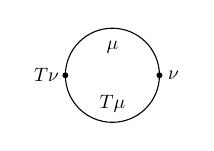
\begin{tikzpicture}[scale=.85]
\draw (0,0) circle (20pt);
\node[scale=.7] at (0,12pt){$\mu$};
\node[scale=.7] at (0,-12pt){$T \mu$};
\node[scale=.7] at (-28pt,0){$T \nu$};
\node[scale=.7] at (26pt,0){$\nu$};
\draw [fill] (-20pt,0) circle [radius=1pt];
\draw [fill] (20pt,0) circle [radius=1pt];
\end{tikzpicture}
\end{equation*}
and let $W^{(0)}$ be the subcomplex generated by $\nu$. We think of $W^{(1)}$ as an $\S_2$-equivariant 1-cell with boundary $W^{(0)}$.

We regard these complexes as $\S$-bimodules concentrated in biarity $(2,1)$, and let $\varphi \colon W^{(0)} \to \A$ be define by sending $T \nu$ and $\nu$ respectively to
\begin{equation*}
\begin{tikzpicture}[scale=.2]
\draw (-4,0)--(-4,4);
\draw (-6,0)--(-6,4);
\draw [fill] (-6,.2) circle [radius=.2];
\node [left] at (-6,0) {$\varepsilon$};

\node at (0,.4) {and};

\draw (4,0)--(4,4);
\draw (6,0)--(6,4);
\draw [fill] (6,.2) circle [radius=.2];
\node [right] at (6,0) {$\varepsilon$.};
\end{tikzpicture}
\end{equation*}
Consider the push-out
\begin{equation*}
\begin{tikzcd}
F(W^{(0)}) \arrow[r, "F(\varphi)"] \arrow[d] & \A \arrow[d, dashed] \\
F(W^{(1)}) \arrow[r, dashed] & \mu \vee_\varphi \A
\end{tikzcd}
\end{equation*}
in the category of props. We think of $\mu \vee_\varphi \A$ as the prop obtained by attaching a $1$-cell in biarity $(2,1)$ to $\A$.

Define $\M$ as the quotient of $\mu \vee_\varphi \A$ by the ideal generated by
\begin{equation*}
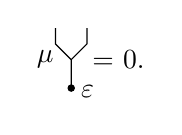
\begin{tikzpicture}[scale=.2]
\draw (5,4)--(5,3)--(6,2)--(6,0);
\draw (7,4)--(7,3)--(6,2);
\node [left] at (5.5,2) {$\mu$};
\draw [fill] (6,.2) circle [radius=.2];
\node [right] at (6,0) {$\varepsilon$};

\node at (9,2) {= 0.};
\end{tikzpicture}
\end{equation*}

We can give a more explicit description of $\M$ using the description of the free prop in terms of $(m,n)$-graphs.
Consider the following elements in $\M$
\begin{equation*}
\counit \in \mathcal M(1,0)_0, \hspace*{.6cm} \coproduct \in \mathcal M(1,2)_0, \hspace*{.6cm} \product \in \mathcal M(2,1)_1,
\end{equation*}
where the decorations by $\varepsilon$, $\Delta$, and $\mu$ are omitted.
Any element in $\M(m,n)$ can be written as a linear combination of the $(m,n)$-graphs generated by these three by grafting, disjoint union and relabeling, modulo the ideals generated by the relations
\begin{equation*}
\qquad \leftcounitality \, , \qquad \rightcounitality \, , \qquad \coassociativity \, , \qquad \productcounit \, .
\end{equation*}
Its chain complex structure is determined using \eqref{e:free prop} by 
\begin{equation*}
\partial\ \counit = 0, \hspace*{.6cm} \partial \ \coproduct = 0, \hspace*{.6cm} \partial \ \product = \ \boundary \, .
\end{equation*}

We have the following results from \cite{Medina20prop1}

\begin{proposition}
	The prop $\M$ is an $E_\infty$-prop.
\end{proposition}

Since $\A$ includes into $\M$, there is a functor $\coAlg_{U(\M)} \to \coAlg_{U(\A)} = \coAlg$.

